\documentclass{beamer}

\setbeamercovered{transparent}

\usepackage{pxfonts}
\usepackage{listings}
\title{Chapter 2: Number Systems and Codes
}
\subtitle{Lesson 2.2: Binary Arithmetic}
\author{Computer Fundamentals}
\institute{Second Edition}
 %\institute{\inst{1}Texas A\&M University \and \inst{2}Other University}
\date{\small{}}

% color
\definecolor{maroon}{RGB}{80,0,0} % A&M's primary color
\definecolor{332C2C}{RGB}{51,44,44} % A&M's primary support color, dark gray
\definecolor{5F574F}{RGB}{95,87,79} % A&M's secondary colors, light gray
\usecolortheme[named=maroon]{structure}
\setbeamercolor{frametitle}{fg=maroon,bg=white}
\setbeamercolor{primary}{fg=white,bg=maroon}
\setbeamercolor{secondary}{fg=white,bg=5F574F}

% headline
\setbeamertemplate{headline}{
\hbox{%
    \begin{beamercolorbox}[wd=0.5\paperwidth,ht=2.25ex,dp=1ex,left]{primary}
        \hspace*{2ex}\insertsectionhead % Section Title in Left
    \end{beamercolorbox}%
    \begin{beamercolorbox}[wd=0.5\paperwidth,ht=2.25ex,dp=1ex,left]{secondary}
        \hspace*{2ex}\insertsubsectionhead % Subsection Title in Right
    \end{beamercolorbox}}
\vskip0pt }

% footline
\setbeamertemplate{footline}{
\hbox{%
    \begin{beamercolorbox}[wd=.49\paperwidth,ht=2.25ex,dp=1ex,left]{primary}
        \hspace*{2ex}{Lesson 1.1: Introduction to Computers} % Something in Left
    \end{beamercolorbox}%
    \begin{beamercolorbox}[wd=.02\paperwidth,ht=2.25ex,dp=1ex,center]{primary}
        %\includegraphics[height=2.25ex,dp=2.25ex]{aTm08-box} % aTm Logo in the Middle
    \end{beamercolorbox}%
    \begin{beamercolorbox}[wd=.49\paperwidth,ht=2.25ex,dp=1ex,right]{primary}
        \insertframenumber{} / \inserttotalframenumber \hspace*{3ex} % Page numbers in Right
    \end{beamercolorbox}}
\vskip0pt }

\let\Tiny=\tiny



\begin{document}
\frame{\titlepage}

\section{Objectives}
\frame{
On completion of this lesson you will know:
\begin{itemize}
  \item Basic concepts of binary arithmetic
\item	Details of step by step binary addition, subtraction, multiplication and division\pause
\item	Additive method of binary subtraction
\end{itemize}
}
\section{Binary Addition }
\frame
{\frametitle {Binary Addition Rule}
Two input binary addition
\begin{tabular}{|c|c|c|c|}
        \hline
        % after \\: \hline or \cline{col1-col2} \cline{col3-col4} ...
        Input &Input 2&Sum &Carry \\ \hline
        0 & 0&0&0 (No Carry)\\ \hline
        0 & 1&0&0 (No Carry)\\ \hline
        1 & 0&0&0 (No Carry)\\ \hline
        1 & 1& 0& 1 (Carry)\\ \hline
        \end{tabular}

Three input binary addition
\begin{tabular}{|c|c|c|c|c|}
        \hline
        % after \\: \hline or \cline{col1-col2} \cline{col3-col4} ...
        Input &Input 2 &Input 3&Sum &Carry \\ \hline
        1 & 1&1&0&1 \\ \hline
        \end{tabular}

}


\frame
{\frametitle {Binary Addition Rule}
Addition of the binary numbers involves the following steps-
\begin{enumerate}
  \item Start addition by adding the bits in unit column (the rightmost column). Use the rules of binary addition.
  \item The result of adding bits of a column is a sum with or without a carry.
  \item Write the sum in the result of that column. If carry is present, the carry is carried-over to the addition of the next left column.
  \item Repeat steps 2-4 for each column and so on.
\end{enumerate}
}


\frame
{\frametitle {Example 2.2.1}
Add 10 and 01. Verify the answer with the help of decimal addition. 
\begin{figure}[!ht]
\centering
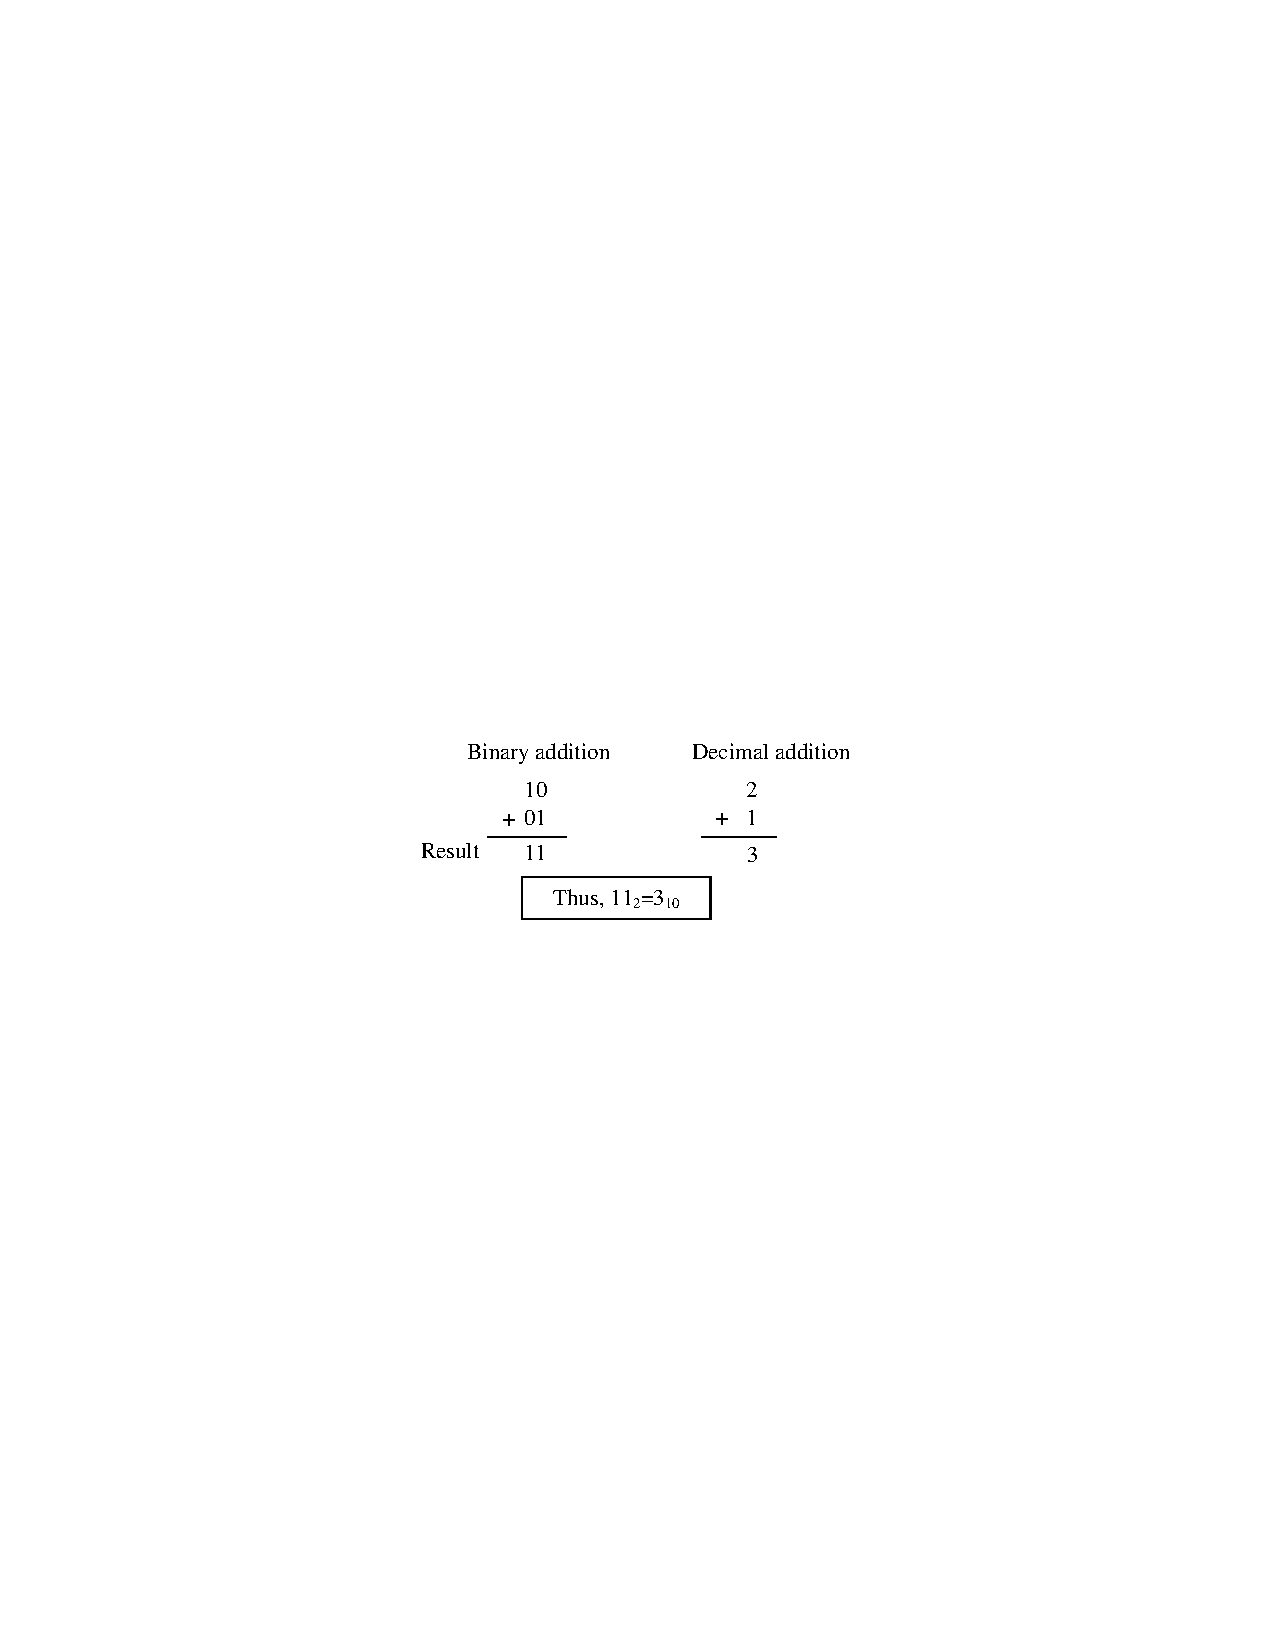
\includegraphics[width=3in]{221}
\end{figure}
}

\frame
{\frametitle {Example 2.2.2}
Add 01 and 11. Verify the answer with the help of decimal addition.
\begin{figure}[!ht]
\centering
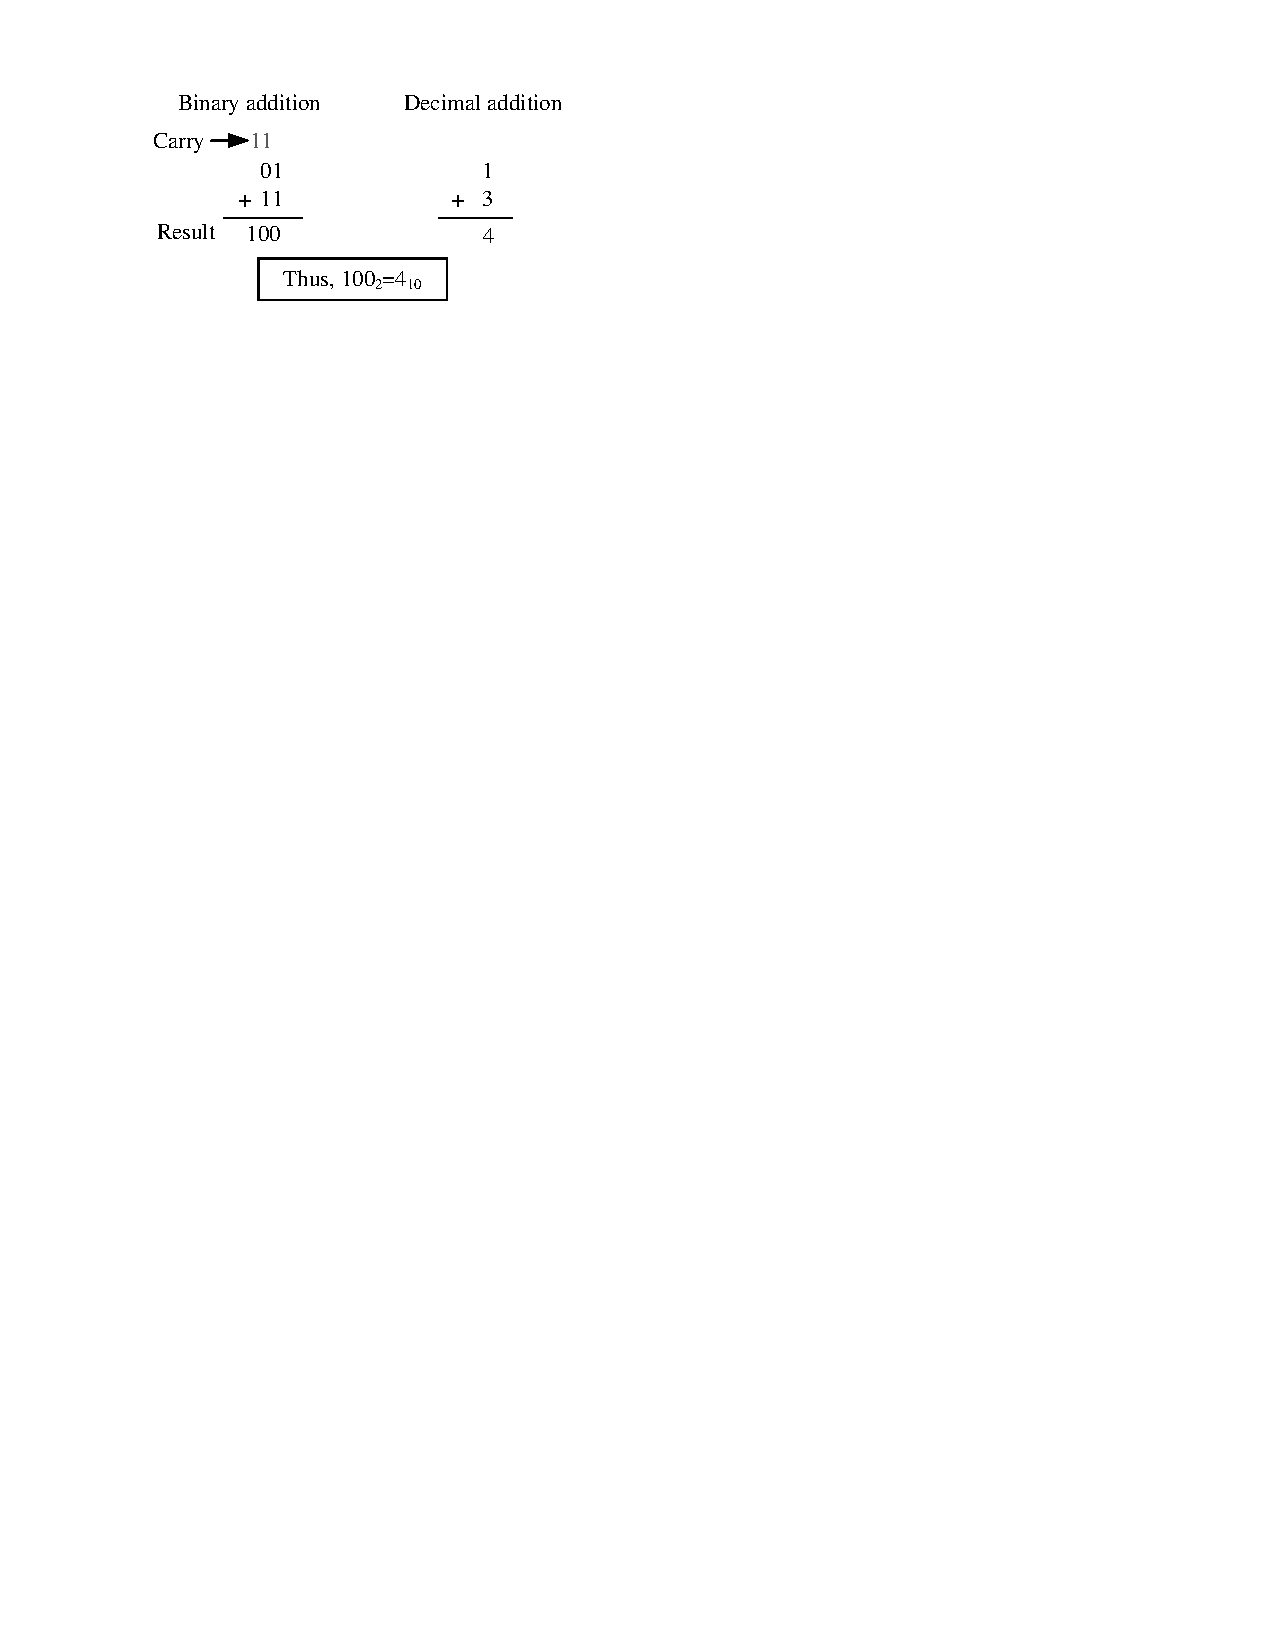
\includegraphics[width=3in]{222}
\end{figure}
}

\frame
{\frametitle {Example 2.2.3}
Add 11 and 11. Verify the answer with the help of decimal addition.
\begin{figure}[!ht]
\centering
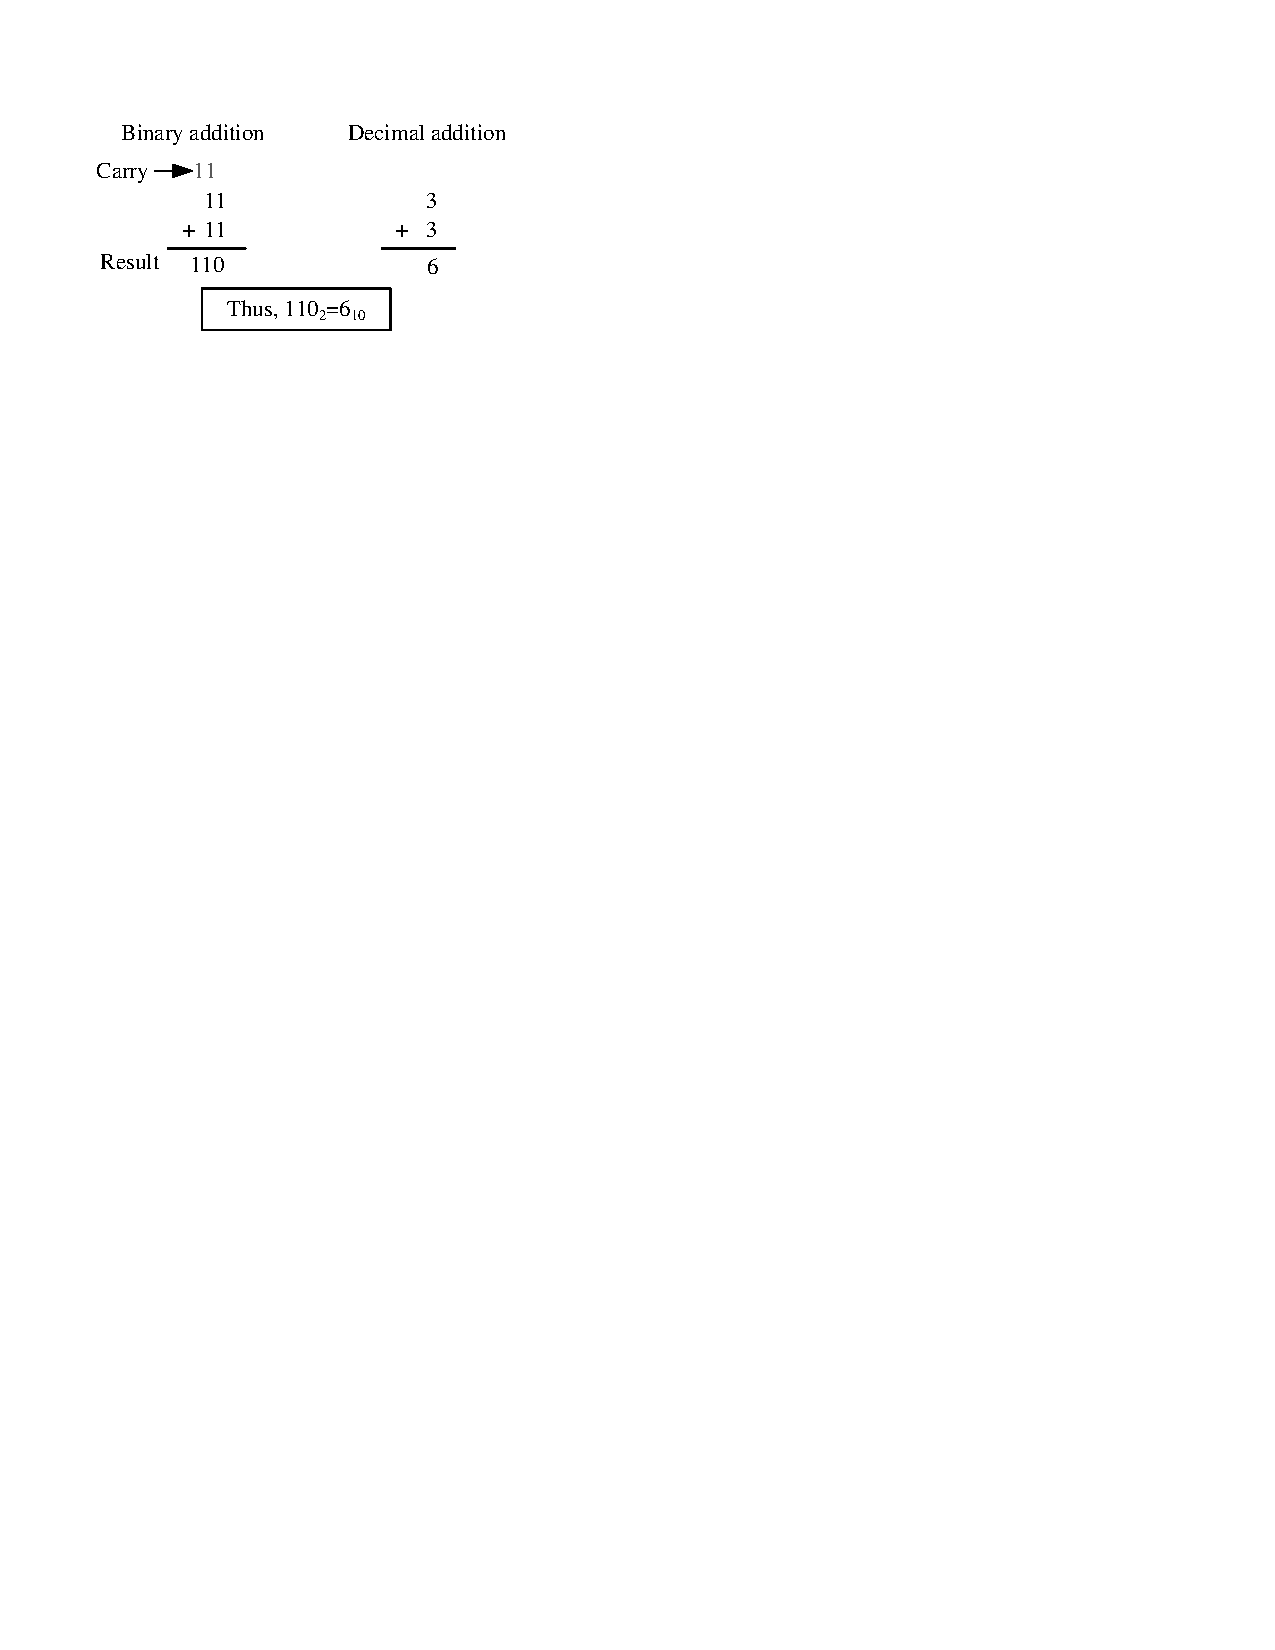
\includegraphics[width=3in]{223}
\end{figure}
}

\frame
{\frametitle {Example 2.2.4}
Add 10111, 11100 and 11. Verify the answer with the help of decimal addition.
\begin{figure}[!ht]
\centering
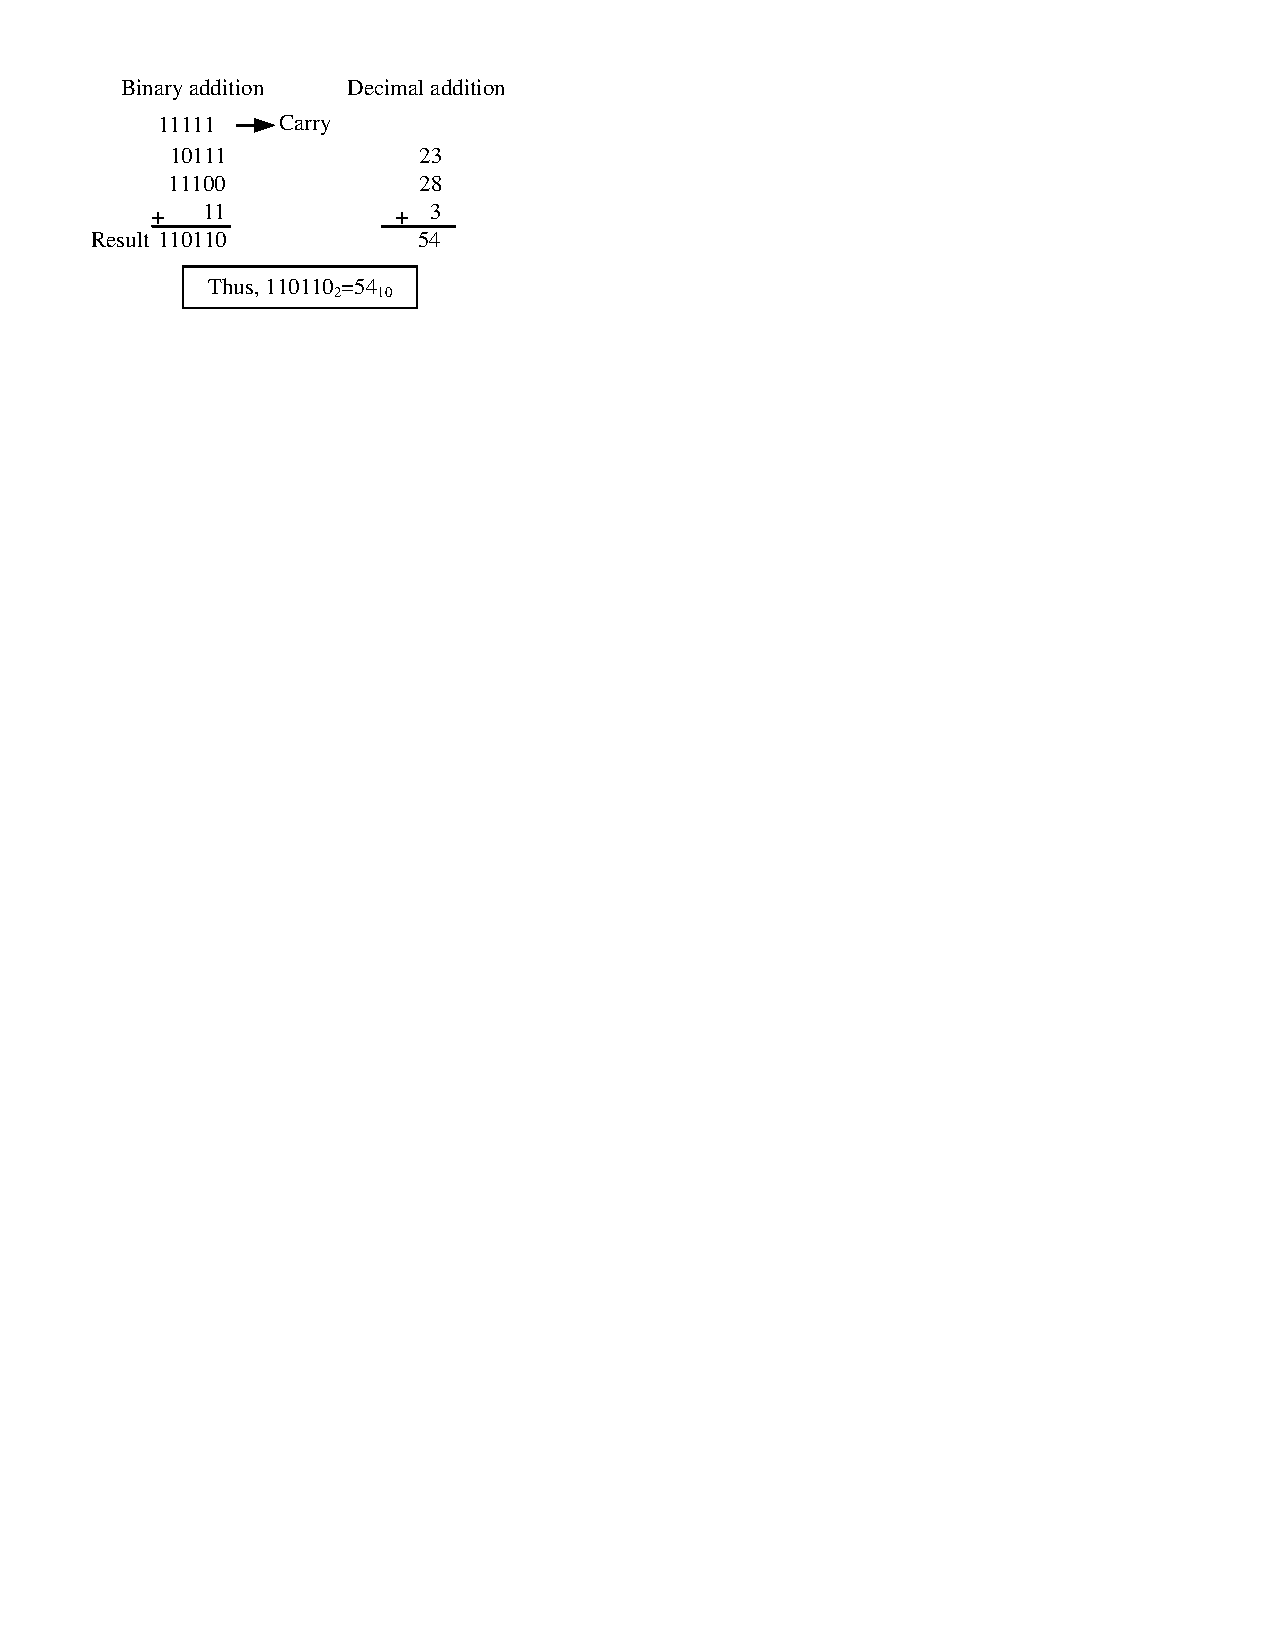
\includegraphics[width=3in]{224}
\end{figure}
}


\section{Binary Substraction}

\frame
{\frametitle {Binary Subtraction Rule}
Two input binary subtraction
\begin{tabular}{|c|c|c|c|}
        \hline
        % after \\: \hline or \cline{col1-col2} \cline{col3-col4} ...
        Input &Input 2&Difference &Borrow \\ \hline
        0 & 0&0&0 (No Borrow)\\ \hline
        0 & 1&1&1 (Borrow)\\ \hline
        1 & 0&1&0 (No Borrow)\\ \hline
        1 & 1& 0&0 (No Borrow)\\ \hline
        \end{tabular}
}

\frame {\frametitle {Binary Subtraction Rule}

The steps for performing subtraction of the binary numbers are as follows
\begin{enumerate}
  \item Start subtraction by subtracting the bit in the lower row from the upper row, in the unit column.
  \item Use the binary subtraction rules. If the bit in the upper row is less than lower row, borrow 1 from the upper row of the next column (on the left side). The result of subtraction of two bits is the difference.
  \item Write the difference in the result of that column.
  \item Repeat step 2-3 for each column and so on.

\end{enumerate}
}

\frame
{\frametitle {Example 2.2.5}
Subtract 01 from 11. Verify the answer with the help of decimal subtraction.
\begin{figure}[!ht]
\centering
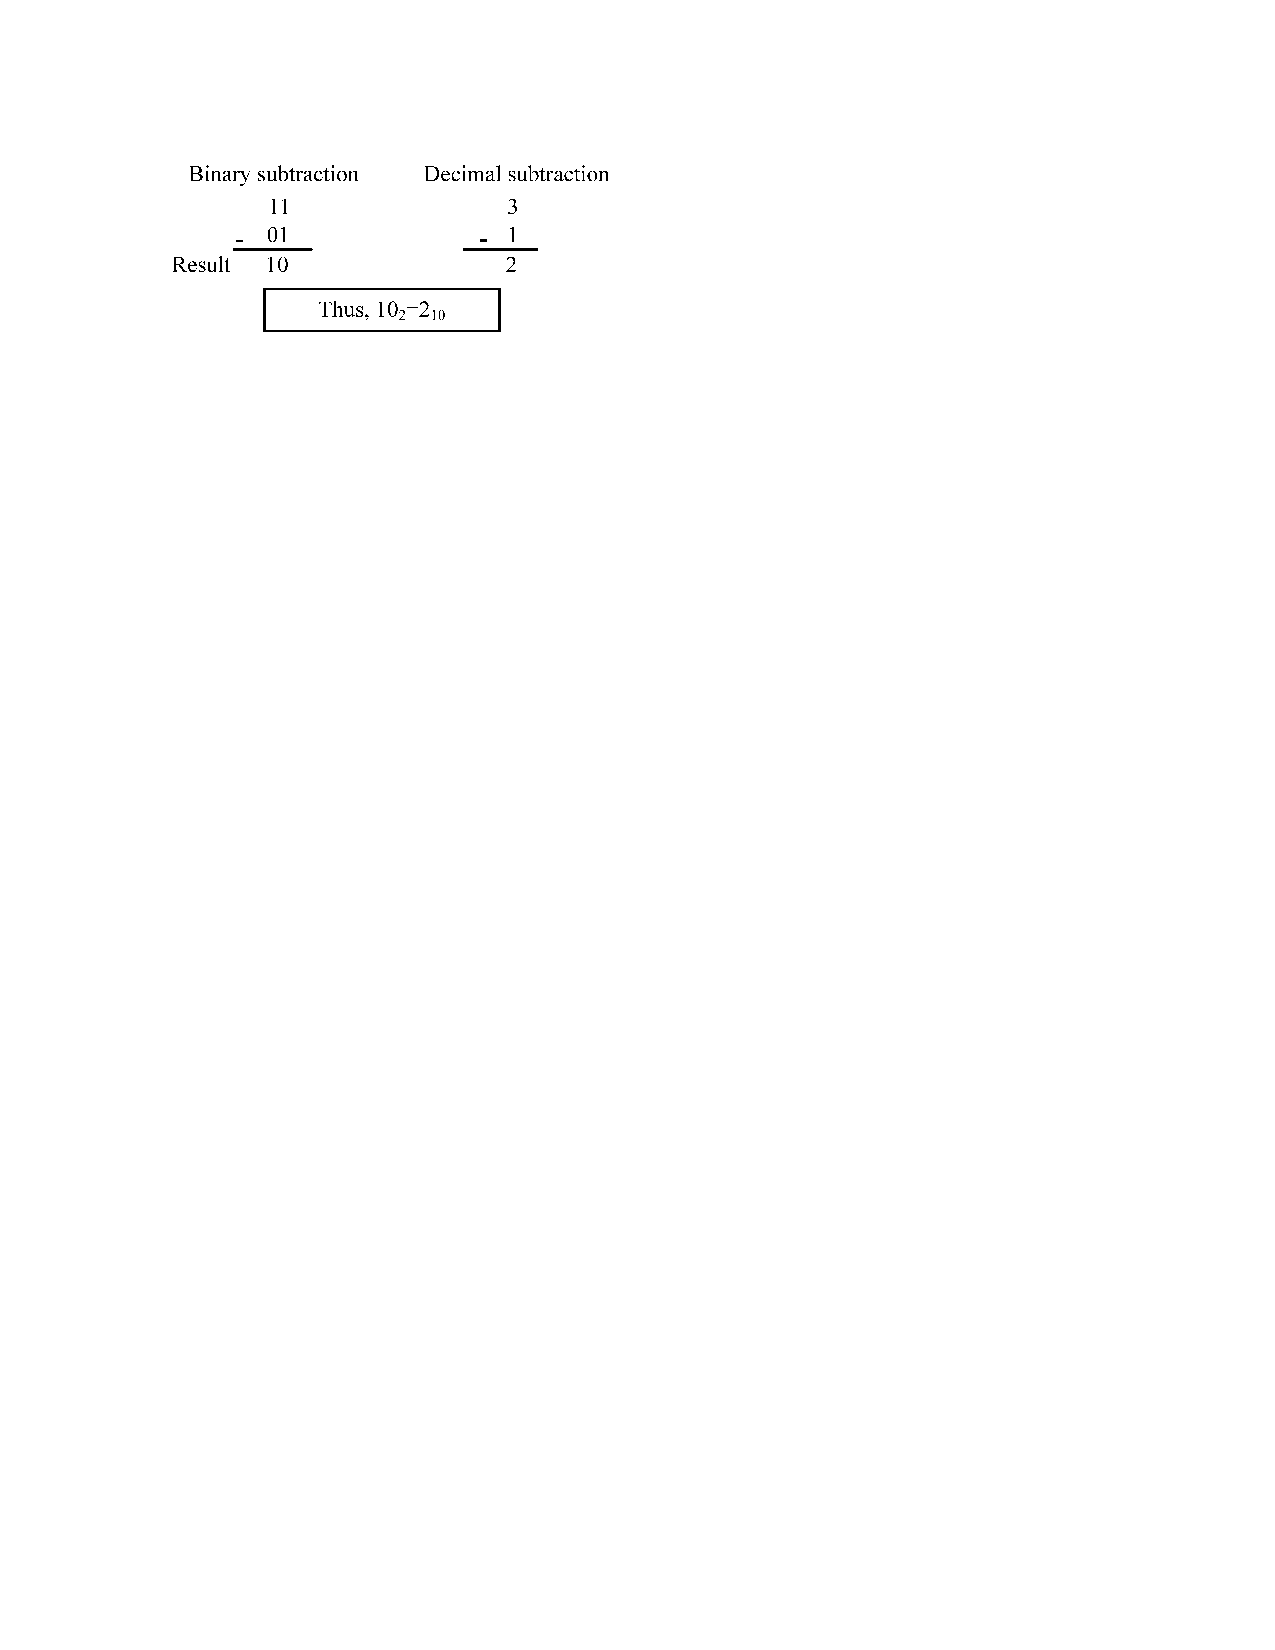
\includegraphics[width=3in]{225}
\end{figure}
}

\frame
{\frametitle {Example 2.2.6}
Subtract 10011111 from 10101001. Verify the answer with the help of decimal subtraction.

\begin{figure}[!ht]
\centering
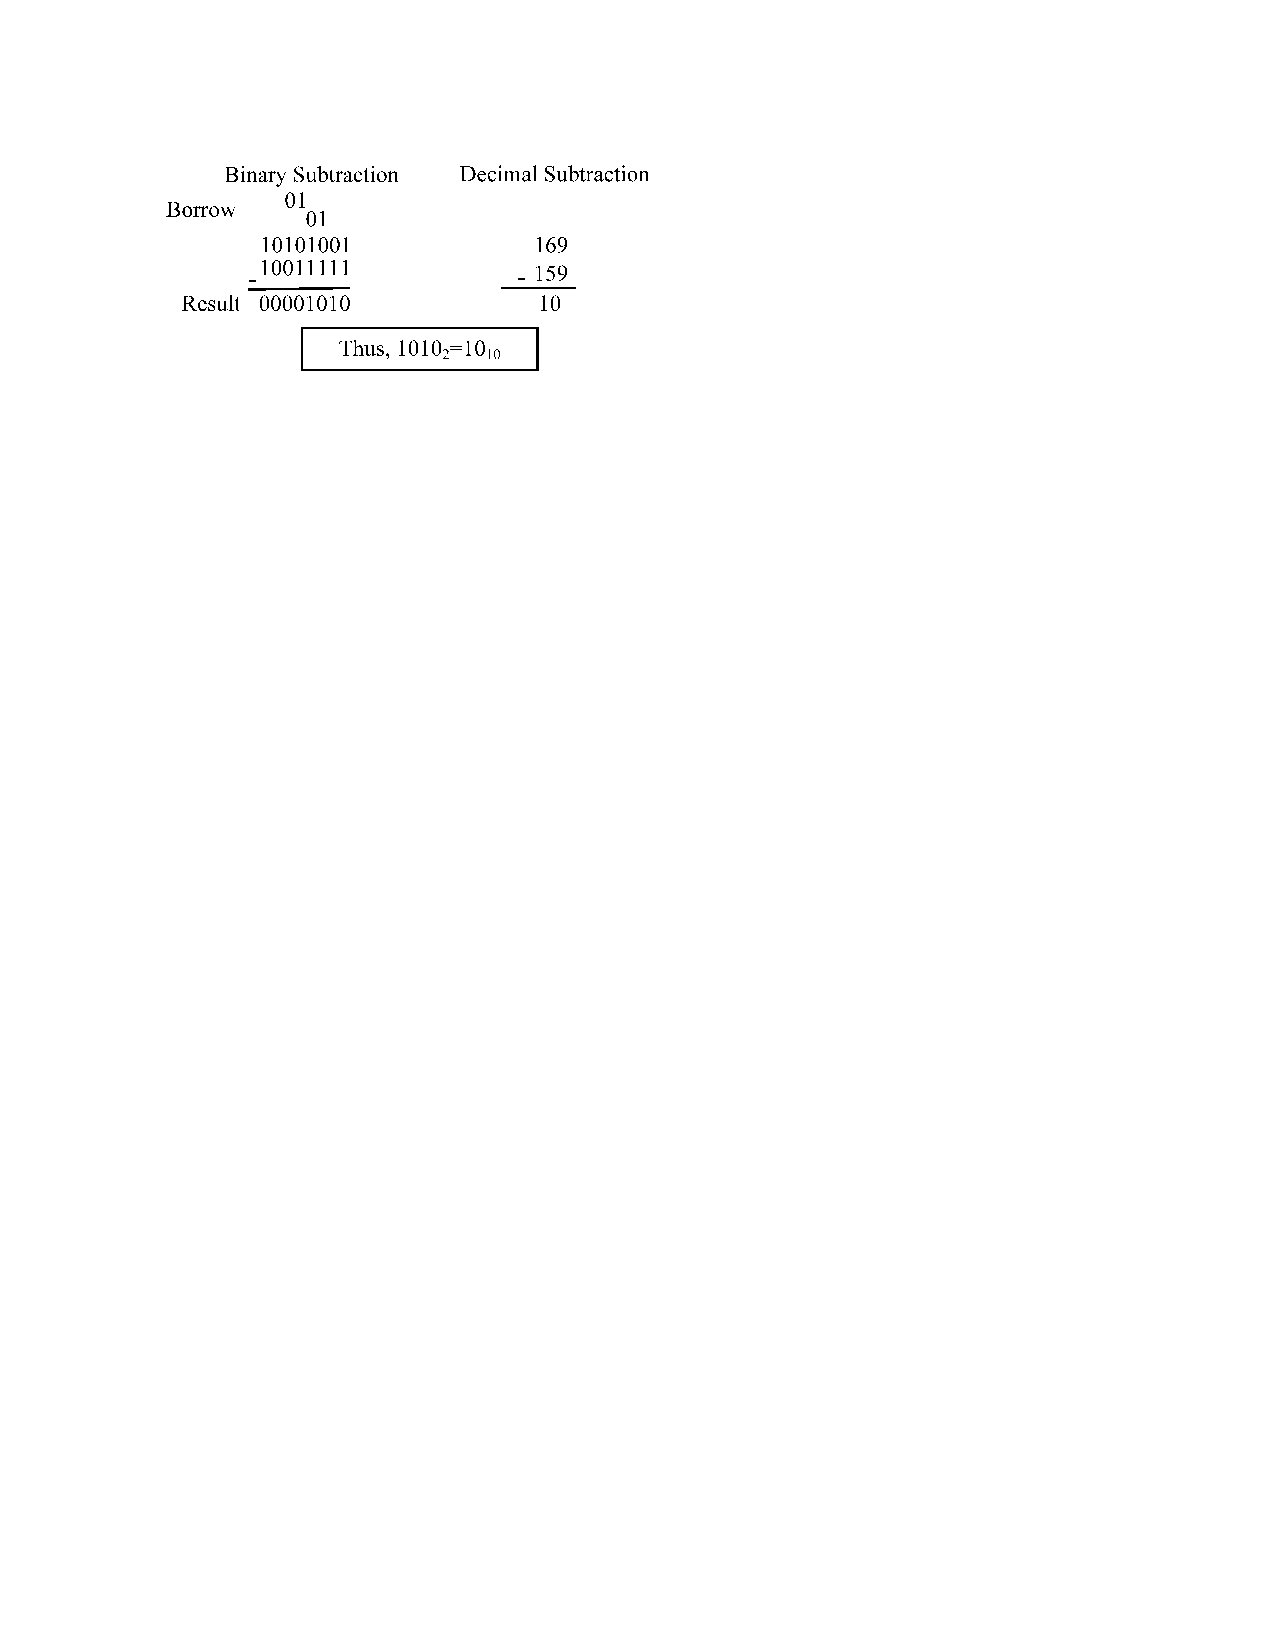
\includegraphics[width=3in]{226}
\end{figure}
}

\frame{
\frametitle{Additive Method of Binary Subtraction}
Additive Method of Binary Subtraction: This method is called complement method. The following steps are involved:
\begin{itemize}
  \item Find the complement of subtrahend.
  \item Add results of step 1 to the minuend.
  \item If a carry is obtained, add it to obtain the result, else recomplement the sum and attach a negative sign to obtain the result.
\end{itemize}
}

\frame
{\frametitle {Example 2.2.7}
Subtract 110111 from 11001 using additive approach. 

\begin{figure}[!ht]
\centering
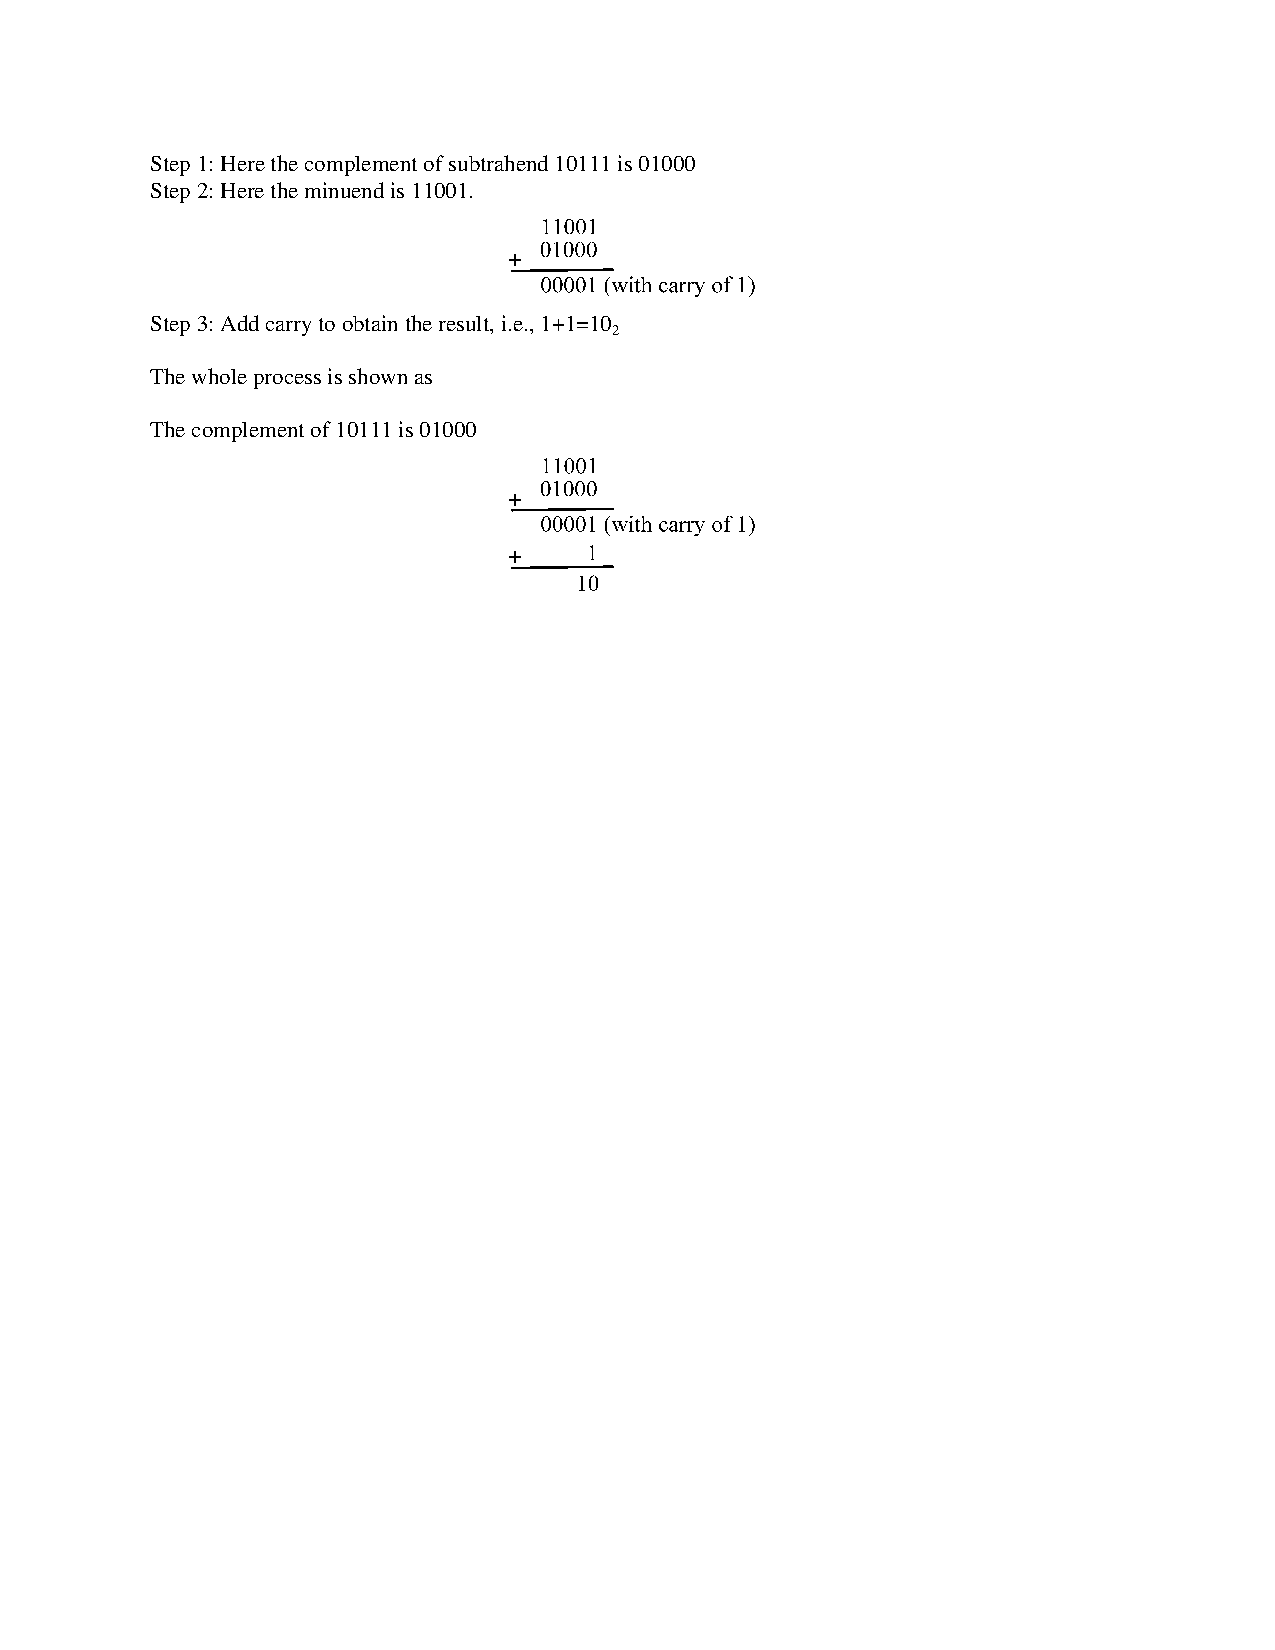
\includegraphics[width=3in]{227}
\end{figure}
}



\section{Binary Multiplication}
\frame {It is actually much simpler than decimal multiplication. In the case of decimal multiplication, we need to remember $3\times 9 = 27$, $7\times 8 = 56$, and so on.

In binary multiplication, we only need to remember the following Table

\begin{tabular}{|c|c|c|}
        \hline
        % after \\: \hline or \cline{col1-col2} \cline{col3-col4} ...
        Input &Input 2&Multiplication  \\ \hline
        0 & 0&0\\ \hline
        0 & 1&0\\ \hline
        1 & 0&0\\ \hline
        1 & 1& 1\\ \hline
        \end{tabular}
}


\frame
{

\begin{figure}[!ht]
\centering
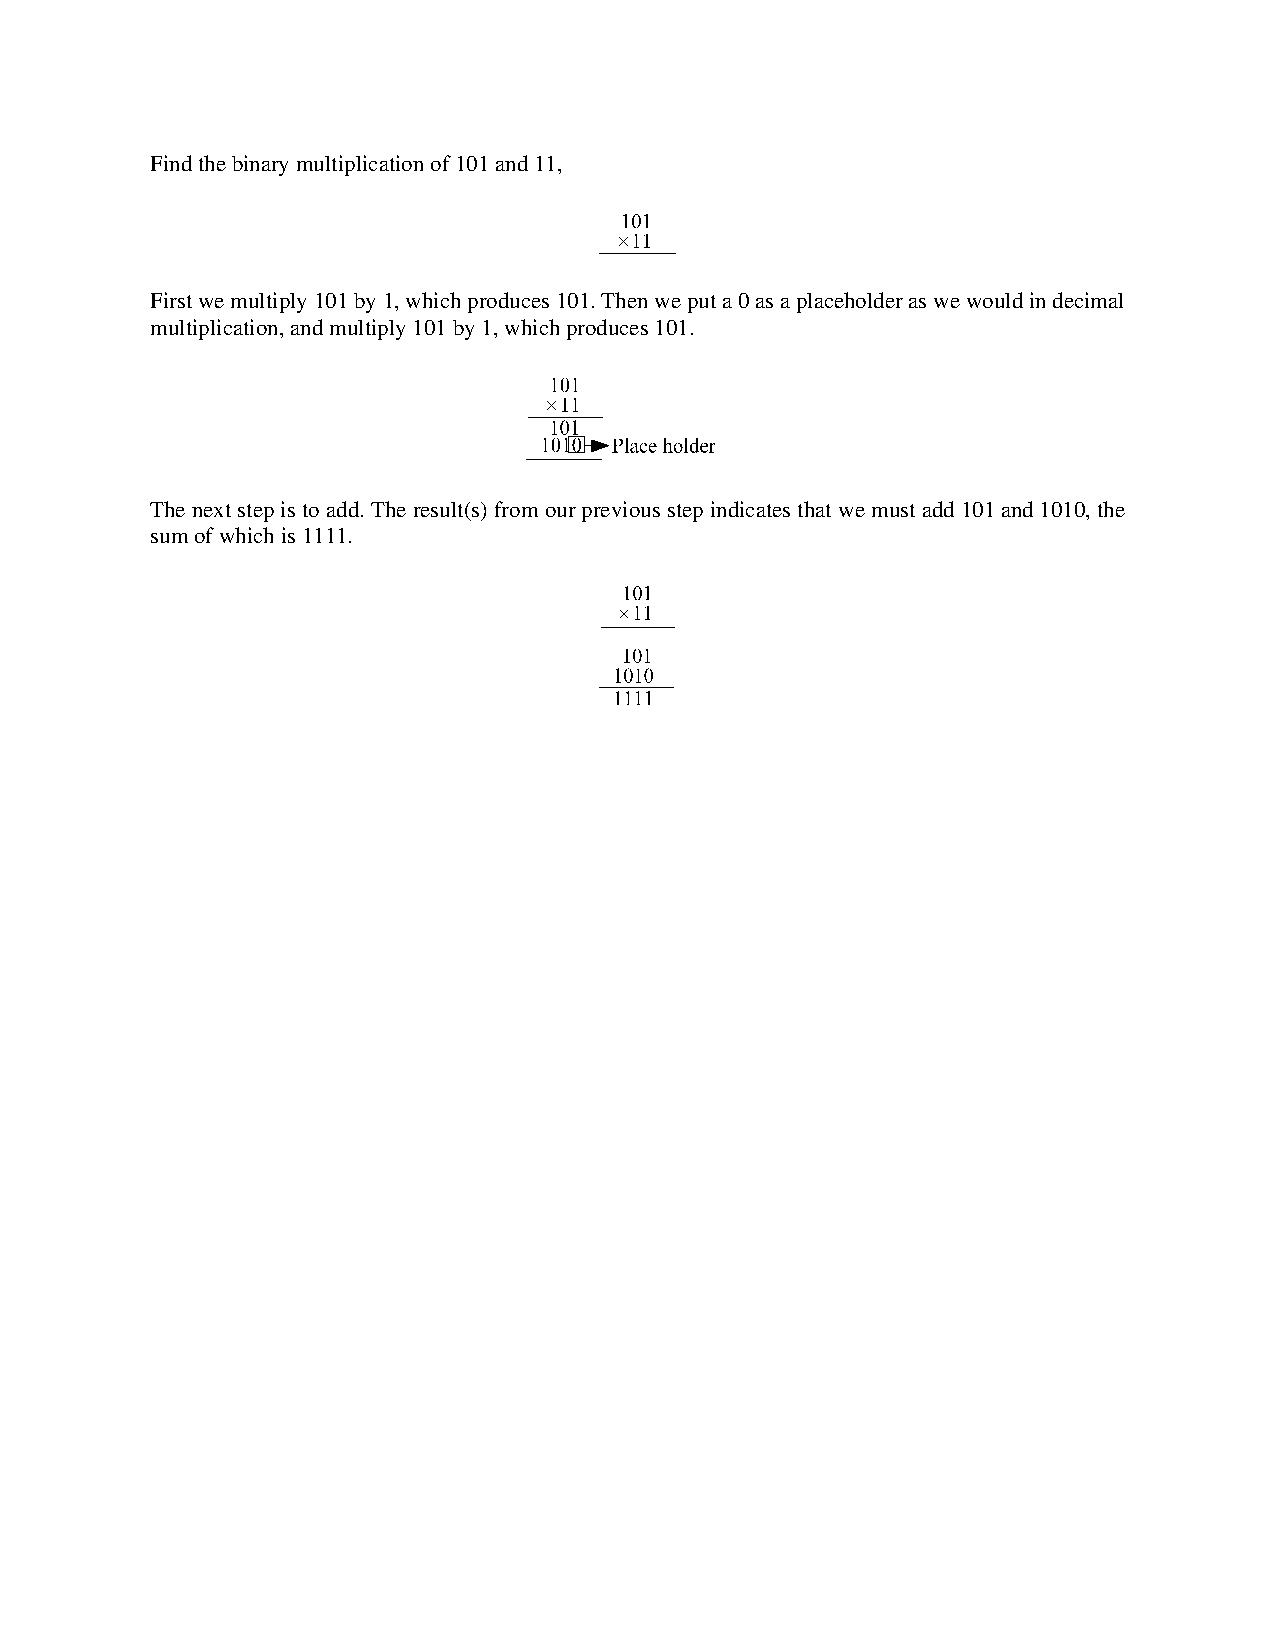
\includegraphics[width=6in]{mul1}
\end{figure}
}

\section{Binary Division}
\frame {\frametitle {Rules for performing binary division}

The method for binary division is as follows:
\begin{itemize}
  \item $\frac{0}{0}=0$
  \item $\frac{1}{1}=1$
\end{itemize}
\begin{enumerate}
  \item Starting from left compare divisor with dividend
  \item If dividend is greater, take value of the quotient 1 and subtract the divisor from the corresponding digits of dividend.
  \item If dividend is less, take value of the quotient 0 and repeat whole process till sufficient digits in dividend
\end{enumerate}
}

\frame
{\frametitle {Example 2.2.9}
Find  $\frac{110011}{101}$

\begin{figure}[!ht]
\centering
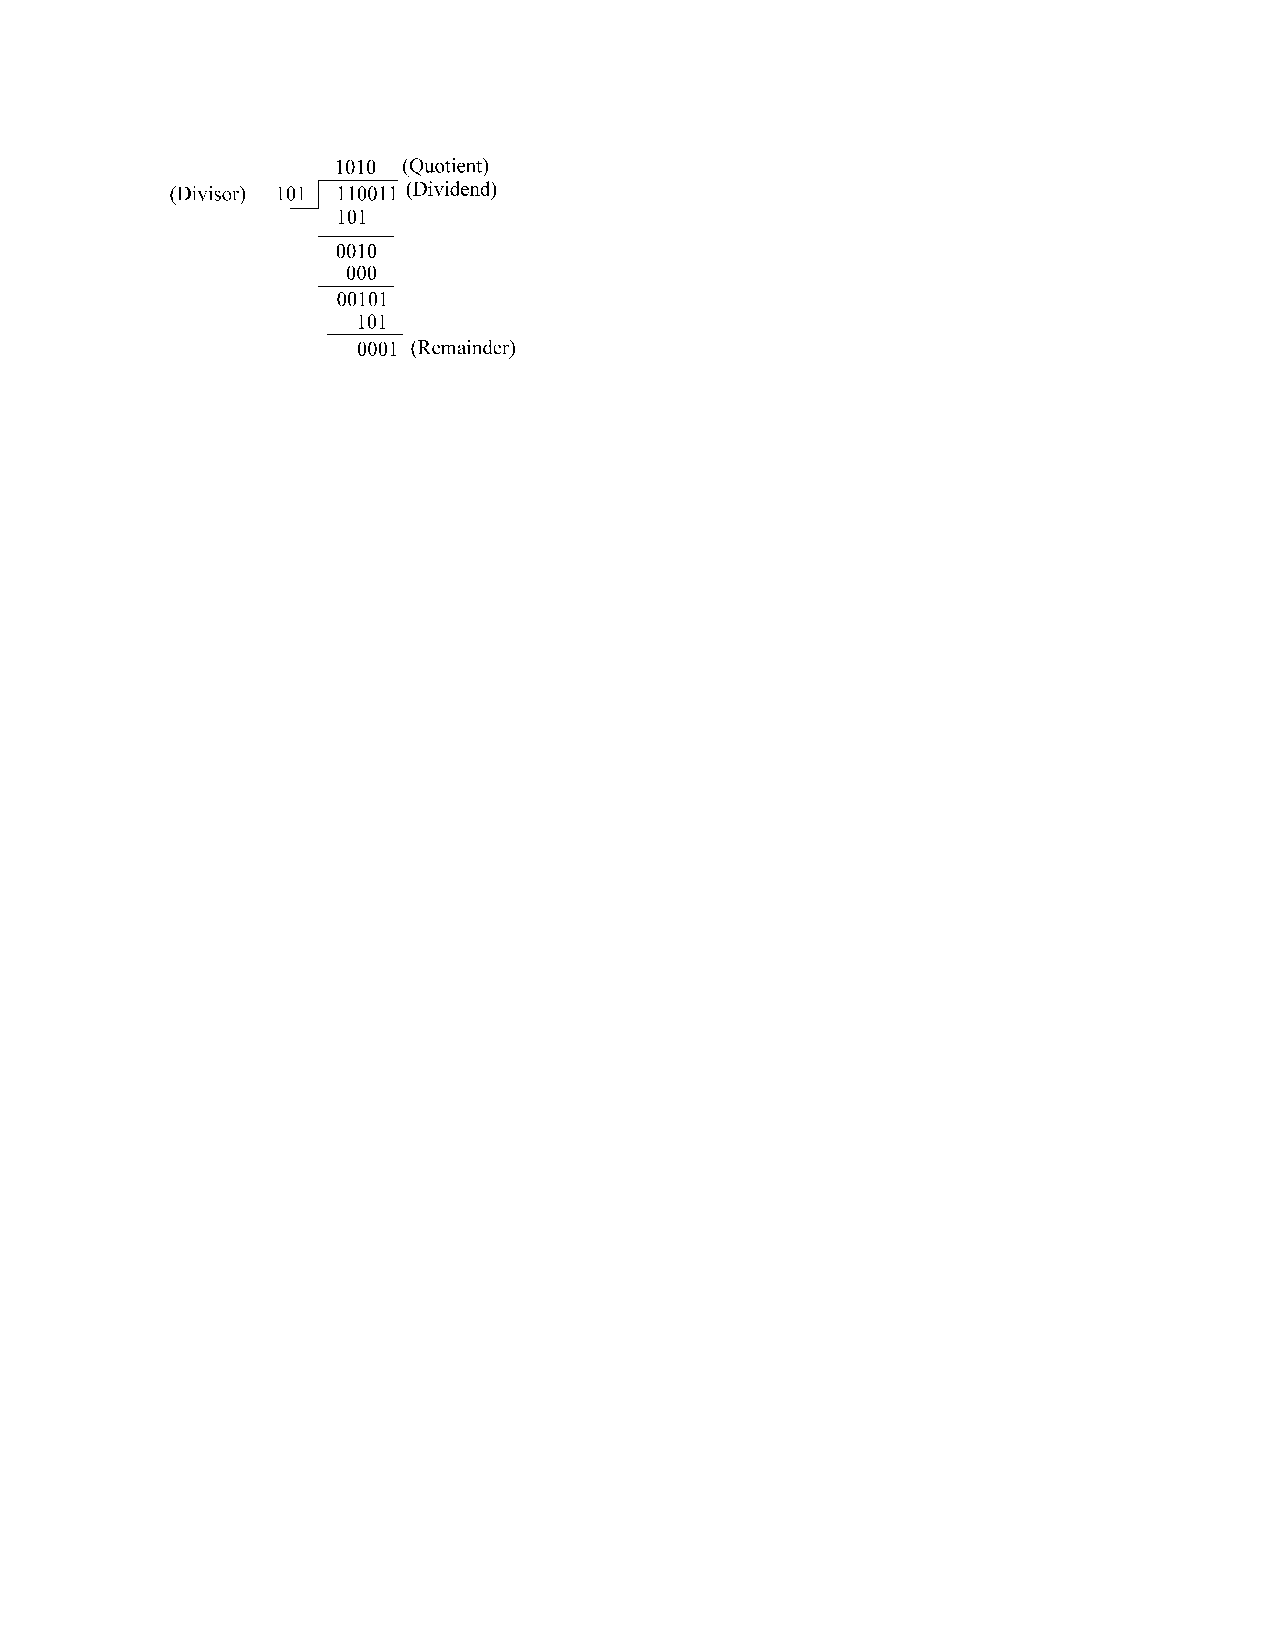
\includegraphics[width=3in]{229}
\end{figure}
}


\end{document}
